% ./dc -meta ./meta -preamble <path_to_latex_preamble> <path_to_tex>

% ./dc -meta ./meta -preamble latex_preamble/preamble.tex ./07_Intro_Graphs/Chapter_07_Intro_Graphs.tex

\chapter{Introduction to Graph Theory}
\label{chapter:intro-to-graph-theory}

\begin{preamble}
In the study of computational complexity of languages and computational problems, graphs play a very fundamental role. This is because an enormous number of computational problems that arise in computer science can be abstracted away as problems on graphs, which model pairwise relations between objects. This is great for various reasons. For one, this kind of abstraction removes unnecessary distractions about the problem and allows us to focus on its essence. Second, there is a huge literature on graph theory, so we can use this arsenal to better understand the computational complexity of graph problems. Applications of graphs are too many and diverse to list here, but we'll name a few to give you an idea: communication networks, finding shortest routes in various settings, finding matchings between two sets of objects, social network analysis, kidney exchange protocols, linguistics, topology of atoms, and compiler optimization.

Our goal in this chapter is to introduce you to graph theory by providing the basic definitions and some well-known graph algorithms.
\end{preamble}



\section{Basic Definitions}



\begin{flex}
\begin{definition}[Undirected graph] \label{definition:Undirected-graph}
An \defn{undirected graph}\footn{Often the word ``undirected'' is omitted.} $G$ is a pair $(V,E)$, where 
\begin{itemize}
    \item $V$ is a finite non-empty set called the set of \defn{vertices} (or \defn{nodes}),
    \item $E$ is a set called the set of \defn{edges}, and every element of $E$ is of the form $\{u,v\}$ for distinct $u, v \in V$.
\end{itemize}
\end{definition}

\begin{example}[A graph with $6$ vertices and $4$ edges] \label{example:A-graph-with-6-vertices-and-4-edges}
Let $G=(V,E)$ where $$V = \{v_1,v_2,v_3,v_4,v_5,v_6\}$$ and $$E = \{\{v_1,v_2\},\{v_1,v_3\},\{v_2,v_3\},\{v_4,v_5\}\}.$$ We usually draw graphs in a way such that a vertex corresponds to a dot and an edge corresponds to a line connecting two dots. For example, the graph we have defined can be drawn as follows:
\begin{center}
    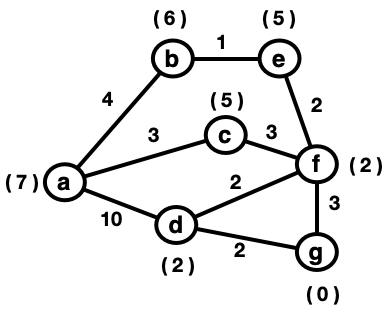
\includegraphics[width=0.4\textwidth]{07_Intro_Graphs/media_upload/graph.png}
\end{center} 
\end{example}
\end{flex}


\begin{note}[$n$ and $m$] \label{note:n-and-m}
Given a graph $G=(V,E)$, we usually use $n$ to denote the number of vertices $|V|$ and $m$ to denote the number of edges $|E|$.
\end{note}


\begin{important}[Representations of graphs] \label{important:Representations-of-graphs}
There are two common ways to represent a graph. Let $v_1,v_2,\ldots,v_n$ be some arbitrary ordering of the vertices. In the \emph{adjacency matrix} representation, a graph is represented by an $n \times n$ matrix $A$ such that
\[ A[i,j] =
  \begin{cases}
    1  & \quad \text{if $\{v_i,v_j\} \in E$,}\\
    0  & \quad \text{otherwise.}\\
  \end{cases}
\]
The adjacency matrix representation is not always the best representation of a graph. In particular, it is wasteful if the graph has very few edges. For such graphs, it can be preferable to use the \emph{adjacency list} representation. In the adjacency list representation, you are given an array of size $n$ and the $i$'th entry of the array contains a pointer to a linked list of vertex $i$'s neighbors.
\end{important}


\begin{flex}
\begin{exercise}[Max number of edges in a graph] \label{exercise:Max-number-of-edges-in-a-graph}
In an $n$-vertex graph, what is the maximum possible value for the number of edges in terms of $n$?
\end{exercise}

\begin{solution}
An edge is a subset of $V$ of size $2$, and there are at most $n \choose 2$ possible subsets of size $2$.
\end{solution}
\end{flex}


\begin{flex}
\begin{definition}[Neighborhood of a vertex] \label{definition:Neighborhood-of-a-vertex}
Let $G=(V,E)$ be a graph, and $e = \{u,v\} \in E$ be an edge in the graph. In this case, we say that $u$ and $v$ are \defn{neighbors} or \defn{adjacent}. We also say that $u$ and $v$ are \defn{incident} to $e$. For $v \in V$, we define the \defn{neighborhood} of $v$, denoted $N(v)$, as the set of all neighbors of $v$, i.e. $N(v) = \{u : \{v,u\} \in E\}$. The size of the neighborhood, $|N(v)|$, is called the \defn{degree} of $v$, and is denoted by $\deg(v)$.
\end{definition}

\begin{example}[Example of neighborhood and degree] \label{example:Example-of-neighborhood-and-degree}
Consider Example~\ref{example:A-graph-with-6-vertices-and-4-edges}. We have $N(v_1) = \{v_2,v_3\}$, $\deg(v_1) = \deg(v_2) = \deg(v_3) = 2$, $\deg(v_4) = \deg(v_5) = 1$, and $\deg(v_6) = 0$.
\end{example}
\end{flex}


\begin{definition}[$d$-regular graphs] \label{definition:d-regular-graphs}
A graph $G = (V,E)$ is called \defn{$d$-regular} if every vertex $v \in V$ satisfies $\deg(v) = d$. 
\end{definition}


\begin{flex}
\begin{theorem}[Handshake Theorem] \label{theorem:Handshake-Theorem}
Let $G=(V,E)$ be a graph. Then 
\[
\sum_{v \in V} \deg(v) = 2m.
\]
\end{theorem}

\begin{proof}
Our goal is to show that the sum of the degrees of all the vertices is equal to twice the number of edges. We will use a \emph{double counting argument} to establish the equality. This means we will identify a set of objects and count its size in two different ways. One way of counting it will give us $\sum_{v \in V} \deg(v)$, and the second way of counting it will give us $2m$. This then immediately implies that $\sum_{v \in V} \deg(v) = 2m$.

We now proceed with the double counting argument. For each vertex $v \in V$, put a ``token'' on all the edges it is incident to. We want to count the total number of tokens. Every vertex $v$ is incident to $\deg(v)$ edges, so the total number of tokens put is $\sum_{v \in V} \deg(v)$. On the other hand, each edge $\{u,v\}$ in the graph will get two tokens, one from vertex $u$ and one from vertex $v$. So the total number of tokens put is $2m$. Therefore it must be that $\sum_{v \in V} \deg(v) = 2m$.
\end{proof}
\end{flex}


\begin{flex}
\begin{exercise}[Application of Handshake Theorem] \label{exercise:Application-of-Handshake-Theorem}
Is it possible to have a party with 251 people in which everyone knows exactly 5 other people in the party?
\end{exercise}

\begin{solution}
Create a vertex for each person in the party, and put an edge between two people if they know each other. Note that the question is asking whether there can be a $5$-regular graph with $251$ nodes. We use Theorem~\ref{theorem:Handshake-Theorem} to answer this question. If such a graph exists, then the sum of the degrees would be $5 \times 251$, which is an odd number. However, this number must equal $2m$ (where $m$ is the number of edges), and $2m$ is an even number. So we conclude that there cannot be a party with 251 people in which everyone knows exactly 5 other people.
\end{solution}
\end{flex}


\begin{definition}[Paths and cycles] \label{definition:Paths-and-cycles}
Let $G=(V,E)$ be a graph. A \defn{path} of length $k$ in $G$ is a sequence of \emph{distinct} vertices $$v_0,v_1,\ldots,v_k$$ such that $\{v_{i-1}, v_i\} \in E$ for all $i \in \{1,2,\ldots,k\}$. In this case, we say that the path is from vertex $v_0$ to vertex $v_k$.

A \defn{cycle} of length $k$ (also known as a $k$-cycle) in $G$ is a sequence of vertices $$v_0, v_1, \ldots, v_{k-1}, v_0$$ such that $v_0, v_1, \ldots, v_{k-1}$ is a path, and $\{v_0,v_{k-1}\} \in E$.\footn{In undirected graphs, we require $k > 2$.} In other words, a cycle is just a ``closed'' path. The starting vertex in the cycle is not important. So for example,
$$v_1, v_2, \ldots, v_{k-1},v_0,v_1$$
would be considered the same cycle. Also, if we list the vertices in reverse order, we consider it to be the same cycle. For example, 
$$v_0, v_{k-1}, v_{k-2} \ldots, v_1, v_0$$
represents the same cycle as before.

A graph that contains no cycles is called \defn{acyclic}.
\end{definition}


\begin{definition}[Connected graph, connected component] \label{definition:Connected-graph-connected-component}
Let $G = (V,E)$ be a graph. We say that two vertices in $G$ are \defn{connected} if there is a path between those two vertices. A \defn{connected graph} $G$ is such that every pair of vertices in $G$ is connected.

A subset $S \subseteq V$ is called a \defn{connected component} of $G$ if $G$ restricted to $S$, i.e. the graph $G' = (S, E' = \{\{u,v\} \in E : u,v \in S\})$, is a connected graph, and $S$ is disconnected from the rest of the graph (i.e. $\{u,v\} \not \in E$ when $u \in S$ and $v \not \in S$). Note that a connected graph is a graph with only one connected component.
\end{definition}


\begin{flex}
\begin{theorem}[Min number of edges to connect a graph] \label{theorem:Min-number-of-edges-to-connect-a-graph}
Let $G = (V,E)$ be a connected graph with $n$ vertices and $m$ edges. Then $m \geq n-1$. Furthermore, $m = n-1$ if and only if $G$ is acyclic.
\end{theorem}

\begin{proof}
We first prove that a connected graph with $n$ vertices and $m$ edges satisfies $m \geq n-1$. Take $G$ and remove all its edges. This graph consists of isolated vertices and therefore contains $n$ connected components. Let's now imagine a process in which we put back the edges of $G$ one by one. The order in which we do this does not matter. At the end of this process, we must end up with just one connected component since $G$ is connected. When we put back an edge, there are two options. Either 
\begin{enumerate}
    \item we connect two different connected components by putting an edge between two vertices that are not already connected, or
    \item we put an edge between two vertices that are already connected, and therefore create a cycle.
\end{enumerate}
Observe that if (1) happens, then the number of connected components goes down by 1. If (2) happens, the number of connected components remains the same. So every time we put back an edge, the number of connected components in the graph can go down by at most 1. Since we start with $n$ connected components and end with $1$ connected component, (1) must happen at least $n-1$ times, and hence $m \geq n-1$. This proves the first part of the theorem. We now prove $m = n-1 \Longleftrightarrow  \text{$G$ is acyclic}$.

$m = n-1 \implies \text{$G$ is acyclic}$: If $m = n-1$, then (1) must have happened at each step since otherwise, we could not have ended up with one connected component. Note that (1) cannot create a cycle, so in this case, our original graph must be acyclic. 

$\text{$G$ is acyclic} \implies m = n-1$: To prove this direction (using the contrapositive), assume $m > n-1$. We know that (1) can happen at most $n-1$ times. So in at least one of the steps, (2) must happen. This implies $G$ contains a cycle.
\end{proof}
\end{flex}



\begin{definition}[Tree, leaf, internal node] \label{definition:Tree-leaf-internal-node}
A graph satisfying two of the following three properties is called a \defn{tree}: 
\begin{enumerate}
    \item connected, 
    \item $m = n-1$, 
    \item acyclic.
\end{enumerate}
A vertex of degree 1 in a tree is called a \defn{leaf}. And a vertex of degree more than 1 is called an \defn{internal node}.
\end{definition}


\begin{flex}
\begin{exercise}[Equivalent definitions of a tree] \label{exercise:Equivalent-definitions-of-a-tree}
Show that if a graph has two of the properties listed in Definition~\ref{definition:Tree-leaf-internal-node}, then it automatically has the third as well.
\end{exercise}

\begin{solution}
If a graph is connected and satisfies $m = n-1$, then it must be acyclic by Theorem~\ref{theorem:Min-number-of-edges-to-connect-a-graph}. If a graph is connected and acyclic, then it must satisfy $m = n-1$, also by Theorem~\ref{theorem:Min-number-of-edges-to-connect-a-graph}. So all we really need to prove is if a graph is acyclic and satisfies $m=n-1$, then it is connected. For this we look into the proof of Theorem~\ref{theorem:Min-number-of-edges-to-connect-a-graph}. If the graph is acyclic, this means that \emph{every time} we put back an edge, we put one that satisfies (1) (here ``(1)'' is referring to the item in the proof of Theorem~\ref{theorem:Min-number-of-edges-to-connect-a-graph}). This is because any edge that satisfies (2) creates a cycle. Every time we put an edge satisfying (1), we reduce the number of connected components by 1. Since $m = n-1$, we put back $n-1$ edges. This means we start with $n$ connected components ($n$ isolated vertices), and end up with $1$ connected component once all the edges are added back. So the graph is connected.
\end{solution}
\end{flex}


\begin{flex}
\begin{exercise}[A tree has at least 2 leaves] \label{exercise:A-tree-has-at-least-2-leaves}
Let $T$ be a tree with at least $2$ vertices. Show that $T$ must have at least $2$ leaves.
\end{exercise}

\begin{solution}
We use Theorem~\ref{theorem:Handshake-Theorem} to prove this (i.e. $\sum_v \deg(v) = 2m$). If a tree has less than 2 leaves, then the sum of the degrees of the vertices would be \emph{at least} $$1 + 2(n-1) = 2n - 1$$ because in the worst-case, we have 1 leaf and $n-1$ vertices with degree $2$ (this is where we use the assumption that $n \geq 2$). The sum of the degrees must equal $2m$, which is always equal to $2(n-1) = 2n - 2$ in a tree. This is a contradiction since $2n-1 > 2n-2$.
\end{solution}
\end{flex}


\begin{flex}
\begin{exercise}[Max degree is at most number of leaves] \label{exercise:Max-degree-is-at-most-number-of-leaves}
Let $T$ be a tree with $L$ leaves. Let $\Delta$ be the largest degree of any vertex in $T$. Prove that $\Delta \leq L$.
\end{exercise}

\begin{solution}
It is instructive to read all 3 proofs.

\noindent
\emph{Proof 1:} We use Theorem~\ref{theorem:Handshake-Theorem}. The degree sum in a tree is always $2n - 2$ since $m = n-1$. Let $v$ be the vertex with maximum degree $\Delta$. The vertices that are not $v$ or leaves must have degree at least $2$ each, so the degree sum is \emph{at least} $\deg(v) + L + 2(n - L - 1)$. So we must have $2n - 2  \geq \deg(v) + L + 2(n - L - 1)$, which simplifies to $L \geq \deg(v) = \Delta$, as desired.

\noindent
\emph{Proof 2:} We induct on the number of vertices. For $n \leq 3$, this follows by inspecting the unique tree on $n$ vertices. For $n > 3$, pick an arbitrary leaf $u$ and delete it (and the edge incident to $u$). Let $T - u$ denote this graph, which is a tree (it is connected and acyclic). Also, we let $L(T)$ denote the number of leaves in $T$ and $L(T-u)$ to denote the number of leaves in $T-u$. We make similar definitions for $\Delta(T)$ and $\Delta(T-u)$ regarding the maximum degrees. Note that  $L(T) \geq L(T - u)$. There are two cases to consider:
\begin{enumerate}
    \item $\Delta(T - u) = \Delta(T)$ 
    \item $\Delta(T - u) = \Delta(T) - 1$
\end{enumerate}
If case 1 happens, then by the induction hypothesis $L(T - u) \geq \Delta(T-u) = \Delta(T)$. But this implies $L(T) \geq \Delta(T)$ (since $L(T) \geq L(T - u)$), as desired.

Let $v$ be the neighbor of $u$. If case 2 happens, then $v$ is the only vertex of maximum degree in $T$. In particular, $v$ cannot be a leaf in $T-u$. So $L(T) = L(T - u) + 1$. The induction hypothesis yields $L(T - u) \geq \Delta(T-u) = \Delta(T) - 1$. Combining this with $L(T) = L(T - u) + 1$ we get $L(T) \geq \Delta(T)$, as desired.

\noindent
\emph{Proof 3:} Let $v$ be a vertex in the tree such that $\deg(v) = \Delta.$ Consider the graph $T - v$ obtained by deleting $v$ and all the edges incident to it. Since $T$ is a tree, we know that $T-v$ contains $\Delta$ connected components; let us denote them $T_1,\ldots, T_{\Delta}$.  Since $T$ is acyclic, each of the $T_i$'s are also acyclic. Since each $T_i$ is connected and acyclic, each one is a tree. There are two possibilities for each $T_i$:
\begin{enumerate}
    \item $T_i$ consists of a single vertex. Then that vertex is a leaf in $T$.
    \item $T_i$ is not a single vertex, and so has at least $2$ leaves (by Exercise~\ref{exercise:A-tree-has-at-least-2-leaves}). At least one of these leaves is not connected to $v$ and therefore must be a leaf in $T$.
\end{enumerate} 
In either case, one vertex in $T_i$ is a leaf in $T$. This is true for all $T_1, \ldots, T_{\Delta}$. Hence we have at least $\Delta$ leaves in $T$.
\end{solution}
\end{flex}


\begin{note}[Root, parent, child, sibling, etc.] \label{note:Root-parent-child-sibling-etc}
Given a tree, we can pick an arbitrary node to be the \emph{root} of the tree. In a rooted tree, we use ``family tree'' terminology: parent, child, sibling, ancestor, descendant, lowest common ancestor, etc. (We assume you are already familiar with these terms.)
\end{note}


\begin{definition}[Directed graph] \label{definition:Directed-graph}
A \defn{directed graph} $G$ is a pair $(V,A)$, where 
\begin{itemize}
    \item $V$ is a non-empty finite set called the set of \emph{vertices} (or \emph{nodes}),
    \item $A$ is a finite set called the set of \emph{directed edges} (or \emph{arcs}), and every element of $A$ is a tuple $(u,v)$ for $u, v \in V$. If $(u,v) \in A$, we say that there is a directed edge from $u$ to $v$. Note that $(u,v) \neq (v,u)$ unless $u = v$.
\end{itemize}
\end{definition}


\begin{note}[Drawing directed graphs] \label{note:Drawing-directed-graphs}
Below is an example of how we draw a directed graph:
\begin{center}
    \includegraphics[width=0.3\textwidth]{07_Intro_Graphs/media_upload/directed-graph.png}
\end{center}
\end{note}


\begin{definition}[Neighborhood, out-degree, in-degree, sink, source] \label{definition:Neighborhood-out-degree-in-degree-sink-source} 
Let $G = (V,A)$ be a directed graph. For $u \in V$, we define the neighborhood of $u$, $N(u)$, as the set $\{v \in V : (u,v) \in A\}$. The \defn{out-degree} of $u$, denoted $\deg_\text{out}(u)$, is $|N(u)|$. The \defn{in-degree} of $u$, denoted $\deg_\text{in}(u)$, is the size of the set $\{v \in V : (v,u) \in A\}$. A vertex with out-degree 0 is called a \defn{sink}. A vertex with in-degree 0 is called a \defn{source}.
\end{definition}


\begin{note}[Paths and cycles in directed graphs] \label{note:Paths-and-cycles-in-directed-graphs}
The notions of \emph{paths} and \emph{cycles} naturally extend to directed graphs. For example, we say that there is a path from $u$ to $v$ if there is a sequence of distinct vertices $u = v_0,v_1,\ldots,v_k = v$ such that $(v_{i-1}, v_i) \in A$ for all $i \in \{1,2,\ldots,k\}$. 
\end{note}





\section{Graph Algorithms}

\subsection{Graph searching algorithms}


\begin{definition}[Arbitrary-first search (AFS) algorithm] \label{definition:Arbitrary-first-search-AFS-algorithm}
The \defn{arbitrary-first search} algorithm, denoted AFS, is the following generic algorithm for searching a given graph. Below, ``bag'' refers to an arbitrary data structure that allows us to add and retrieve objects. 

\begin{center}
    \includegraphics[width=0.7\textwidth]{07_Intro_Graphs/media_upload/alg-afs.png}
\end{center}

Note that when a vertex $w$ is added to the bag, it gets there because it is the neighbor of a vertex $v$ that has been just marked by the algorithm. In this case, we'll say that $v$ is the \emph{parent} of $w$ (and $w$ is the \emph{child} of $v$). Explicitly keeping track of this parent-child relationship is convenient, so we modify the above algorithm to keep track of this information. Below, a tuple of vertices $(v,w)$ has the meaning that vertex $v$ is the parent of $w$. The initial vertex $s$ has no parent, so we denote this situation by $(\perp, s)$.

\begin{center}
    \includegraphics[width=0.7\textwidth]{07_Intro_Graphs/media_upload/alg-afs-2.png}
\end{center}
\end{definition}


\begin{note}[Traversing all the vertices in the graph] \label{note:Traversing-all-the-vertices-in-the-graph}
Note that AFS($G$, $s$) visits all the vertices in the connected component that $s$ is a part of. If we want to traverse all the vertices in the graph, and the graph has multiple connected components, then we can do:
\begin{center}
    \includegraphics[width=0.7\textwidth]{07_Intro_Graphs/media_upload/alg-afs2.png}
\end{center}
\end{note}


\begin{definition}[Breadth-first search (BFS) algorithm] \label{definition:Breadth-first-search-BFS-algorithm} 
The \defn{breadth-first search} algorithm, denoted BFS, is AFS where the bag is chosen to be a \emph{queue} data structure. 
\end{definition}


\begin{note}[Running time of BFS] \label{note:Running-time-of-BFS} 
The running time of BFS($G,s$) is $O(m)$, where $m$ is the number of edges of the input graph. If we do a BFS for each connected component, the total running time is $O(m+n)$, where $n$ is the number of vertices.\footn{Take a moment to reflect on why this is the case.} (We are assuming the graph is given as an adjacency list.)
\end{note}


\begin{definition}[Depth-first search (DFS) algorithm] \label{definition:Depth-first-search-DFS-algorithm} 
The \defn{depth-first search} algorithm, denoted DFS, is AFS where the bag is chosen to be a \emph{stack} data structure. 
\end{definition}


\begin{note}[Recursive DFS] \label{note:Recursive-DFS}
There is a natural recursive representation of the DFS algorithm, as follows.
\begin{center}
    \includegraphics[width=0.7\textwidth]{07_Intro_Graphs/media_upload/alg-dfs.png}
\end{center}
\end{note}


\begin{note}[Running time of DFS] \label{note:Running-time-of-DFS}
The running time of DFS($G,s$) is $O(m)$, where $m$ is the number of edges of the input graph. If we do a DFS for each connected component, the total running time is $O(m+n)$, where $n$ is the number of vertices. (We are assuming the graph is given as an adjacency list.)
\end{note}


\begin{note}[Search algorithms on directed graphs] \label{note:Search-algorithms-on-directed-graphs}
The search algorithms presented above can be applied to directed graphs as well.
\end{note}






\subsection{Minimum spanning tree}


\begin{definition}[Minimum spanning tree (MST) problem] \label{definition:Minimum-spanning-tree-MST-problem} 
In the \defn{minimum spanning tree problem}, the input is a connected undirected graph $G = (V,E)$ together with a \emph{cost} function $c : E \to \R^+$. The output is a subset of the edges of minimum total cost such that, in the graph restricted to these edges, all the vertices of $G$ are connected.\footn{Obviously this subset of edges would not contain a cycle since if it did, we could remove any edge on the cycle, preserve the connectivity property, and obtain a cheaper set. Therefore, this set forms a tree.} For convenience, we'll assume that the edges have unique edge costs, i.e. $e \neq e' \implies c(e) \neq c(e')$.
\end{definition}


\begin{note}[Unique edges costs imply unique MST] \label{note:Unique-edges-costs-imply-unique-MST}
With unique edge costs, the minimum spanning tree is unique.
\end{note}


\begin{flex}
\begin{theorem}[MST cut property] \label{theorem:MST-cut-property} 
Suppose we are given an instance of the MST problem. For any $V' \subseteq V$, let $e = \{u,w\}$ be the cheapest edge with the property that $u \in V'$ and $w \in V\backslash V'$. Then $e$ must be in the minimum spanning tree.
\end{theorem}

\begin{proof}
Let $T$ be the minimum spanning tree. The proof is by contradiction, so assume that $e = \{u,w\}$ is not in $T$. Since $T$ spans the whole graph, there must be a path from $u$ to $w$ in $T$. Let $e' = \{u',w'\}$ be the first edge on this path such that $u' \in V'$ and $w' \in V \backslash V'$. Let $T_{e-e'} = (T \backslash \{e'\}) \cup \{e\}$. If $T_{e-e'}$ is a spanning tree, then we reach a contradiction because $T_{e-e'}$ has lower cost than $T$ (since $c(e) < c(e')$). 

\begin{center}
    \includegraphics[width=0.35\textwidth]{07_Intro_Graphs/media_upload/mst.png}
\end{center}

$T_{e-e'}$ is a spanning tree: Clearly $T_{e-e'}$ has $n-1$ edges (since $T$ has $n-1$ edges). So if we can show that $T_{e-e'}$ is connected, this would imply that $T_{e-e'}$ is a tree and touches every vertex of the graph, i.e., $T_{e-e'}$ is a spanning tree. Consider any two vertices $s,t \in V$. There is a unique path from $s$ to $t$ in $T$. If this path does not use the edge $e' = \{u',w'\}$, then the same path exists in $T_{e-e'}$, so $s$ and $t$ are connected in $T_{e-e'}$. If the path does use $e' = \{u',w'\}$, then instead of taking the edge $\{u',w'\}$, we can take the following path: take the path from $u'$ to $u$, then take the edge $e = \{u,w\}$, then take the path from $w$ to $w'$. So replacing $\{u',w'\}$ with this path allows us to construct a sequence of vertices starting from $s$ and ending at $t$, such that each consecutive pair of vertices is an edge. Therefore $s$ and $t$ are connected.
\end{proof}
\end{flex}


\begin{flex}
\begin{theorem}[Jarn\'{i}k-Prim algorithm for MST] \label{theorem:Jarnik-Prim-algorithm-for-MST}
There is an algorithm that solves the MST problem in polynomial time.
\end{theorem}

\begin{proof}
We first present the algorithm which is due to Jarn\'{i}k and Prim. Given an undirected graph $G=(V,E)$ and a cost function $c : E \to \R^+$:

\begin{center}
    \includegraphics[width=0.7\textwidth]{07_Intro_Graphs/media_upload/alg-prim.png}
\end{center}

By Theorem~\ref{theorem:MST-cut-property}, the algorithm always adds an edge that must be in the MST. The number of iterations is $n-1$, so all the edges of the MST are added to $E'$. Therefore the algorithm correctly outputs the unique MST. 

The running time of the algorithm can be upper bounded by $O(nm)$ because there are $O(n)$ iterations, and the body of the loop can be done in $O(m)$ time.
\end{proof}
\end{flex}


\begin{flex}
\begin{exercise} [MST with negative costs] \label{exercise:MST-with-negative-costs}
Suppose an instance of the Minimum Spanning Tree problem is allowed to have negative costs for the edges. Explain whether we can use the Jarn\'{i}k-Prim algorithm to compute the minimum spanning tree in this case.
\end{exercise}

\begin{solution}
Yes, we can. Assign a rank to each edge of the graph based on its cost: the highest cost edge gets the highest rank and the lowest cost edge gets the lowest rank. When making its decisions, the Jarn\'{i}k-Prim algorithm only cares about the ranks of the edges, and not the specific costs of the edges. The algorithm would output the same tree even if we add a constant $C$ to the costs of all the edges since this would not change the rank of the edges. And indeed, adding a constant to the cost of each edge does not change what the minimum spanning tree is. Hence, we can turn any instance with negative costs into and equivalent one with non-negative costs by adding a large enough constant to all the edges without changing the tree that is output.

\noindent
(Note: In fact the original algorithm would output the minimum cost spanning tree even if the edge costs are allowed to be negative. There is not even a need to add a constant to the edge costs.)
\end{solution}
\end{flex}


\begin{flex}
\begin{exercise} [Maximum spanning tree] \label{exercise:Maximum-spanning-tree}
Consider the problem of computing the maximum spanning tree, i.e., a spanning tree that maximizes the sum of the edge costs. Explain whether the Jarn\'{i}k-Prim algorithm solves this problem if we modify it so that at each iteration, the algorithm chooses the edge between $V'$ and $V\backslash V'$ with the maximum cost.
\end{exercise}

\begin{solution}
Let $(G,c)$ be the input, where $G = (V,E)$ is a graph and $c: E \to \mathbb{R}^+$ is the cost function. Let $c' : E \to \mathbb{R}^{-}$ be defined as follows: for all $e \in E$, $c'(e) = - c(e)$. Let $A_{\min}$ be the original Jarn\'{i}k-Prim algorithm and let $A_{\max}$ be the Jarn\'{i}k-Prim algorithm where we pick the maximum cost edge in each iteration.  There are a couple of important observations:
\begin{enumerate}
    \item The minimum spanning tree for $(G,c')$ is the maximum spanning tree for $(G,c)$. 
    \item Running $A_{\max}(G,c)$ is equivalent to running $A_{\min}(G,c')$, and they output the same spanning tree. 
\end{enumerate}
From Exercise~\ref{exercise:MST-with-negative-costs}, we know $A_{\min}(G,c')$ gives us a minimum cost spanning tree. So $A_{\max}(G,c)$ gives the correct maximum cost spanning tree.
\end{solution}
\end{flex}


\begin{flex}
\begin{exercise} [Kruskal's algorithm] \label{exercise:Kruskals-algorithm}
Consider the following algorithm for the MST problem (which is known as Kruskal's algorithm). Start with MST being the empty set. Go through all the edges of the graph one by one from the cheapest to the most expensive. Add the edge to the MST if it does not create a cycle. Show that this algorithm correctly outputs the MST.
\end{exercise}

\begin{solution}
We do not have the solution to this problem at this time. But we are happy to discuss it with you during office hours.
\end{solution}
\end{flex}




\subsection{Topological sorting}


\begin{flex}
\begin{definition}[Topological order of a directed graph]
A \emph{topological order} of an $n$-vertex directed graph $G = (V,A)$ is a bijection $f: V \to \{1,2,\ldots,n\}$ such that if $(u,v) \in A$, then $f(u) < f(v)$. 
\end{definition}

\begin{example}[Example of topological order]
On the left, we have a directed graph, and on the right, we represent the topological order of the graph. 
\begin{center}
    \includegraphics[width=0.6\textwidth]{07_Intro_Graphs/media_upload/topological-order.png}
\end{center}
Here, $f(e) = 1$, $f(d) = 2$, $f(a) = 3$, $f(b) = 4$, and $f(c) = 5$.
\end{example}
\end{flex}


\begin{flex}
\begin{exercise}[Cycle implies no topological order]
Show that if a directed graph has a cycle, then it does not have a topological order.
\end{exercise}

\begin{solution}
Let $G=(V,A)$ be a directed graph and suppose $u_1,u_2,\ldots,u_k,u_1$ is a cycle in $G$. This means that for all $i \in \{1,2,\ldots,k-1\}$, $(u_i,u_{i+1}) \in A$, and $(u_k,u_1) \in A$. If there is a topological order $f$ of $G$, then by definition, it must be the case that
\[
f(u_1) < f(u_2) < f(u_3) < \cdots < f(u_k) < f(u_1).
\]
This implies $f(u_1) < f(u_k) < f(u_1)$, which is impossible.
\end{solution}
\end{flex}


\begin{definition}[Topological sorting problem]
In the \emph{topological sorting problem}, the input is a directed acyclic graph, and the output is a topological order of the graph.
\end{definition}


\begin{flex}
\begin{lemma}[Acyclic directed graph has a sink]
If a directed graph is acyclic, then it has a sink vertex.
\end{lemma}

\begin{proof}
By contrapositive: If a directed graph has no sink vertices, then it means that every vertex has an outgoing edge. Start with any vertex, and follow an outgoing edge to arrive at a new vertex. Repeat this process. At some point, you have to visit a vertex that you have visited before. This forms a cycle.
\begin{center}
    \includegraphics[width=0.6\textwidth]{07_Intro_Graphs/media_upload/directed-cycle.png}
\end{center}
\end{proof}
\end{flex}


\begin{note}[Topological sort - na\"{i}ve algorithm]
The following algorithm solves the topological sorting problem in polynomial time.
\begin{center}
    \includegraphics[width=0.7\textwidth]{07_Intro_Graphs/media_upload/alg-naive-top-sort.png}
\end{center}
% \begin{algorithm}
% $G = (V,A)$: directed acyclic graph. \\
% Top-Sort-Naive$(\langle G \rangle)$:
% \begin{steps}
%     \setlength\itemsep{0em}
%     \item[\tiny{1}] $p = |V|$.
%     \item[\tiny{2}] While $p \geq 1$:
%     %\item[\tiny{3}] \quad If a sink vertex does not exist, output False.
%     \item[\tiny{3}] \quad Find a sink vertex $v$ and remove it from $G$.
%     \item[\tiny{4}] \quad $f(v) = p$.
%     \item[\tiny{5}] \quad $p = p-1$.
%     \item[\tiny{6}] Output $f$. 
% \end{steps}
% \end{algorithm}
\end{note}


\begin{flex}
\begin{exercise}[Topological sort, correctness of na\"{i}ve algorithm]
Show the algorithm above correctly solves the topological sorting problem, i.e., show that for $(u,v) \in A$, $f(u) < f(v)$. What is the running time of this algorithm?
\end{exercise}

\begin{solution}
We will use the following observation: if an algorithm removes an edge $(u,v) \in A$, then it must be because $v$ is chosen as a sink vertex and removed from the graph. 

We now prove that the algorithm is correct by a proof by contradiction. Suppose $(u,v) \in A$ such that $f(u) > f(v)$. This means that $u$ was removed from the graph before $v$ was removed. At the moment that $u$ is removed, $u$ must be a sink (i.e. it must not have any outgoing edges). This implies the edge $(u,v)$ must have been removed at a previous iteration. But the only way $(u,v)$ would be removed is if $v$ was chosen to be a sink vertex and removed. This implies that $v$ must have been removed before $u$, which is the desired contradiction.

A straightforward implementation of the algorithm would result in a running time of $O(n^2)$ since the algorithm has $n$ iterations, and in each iteration, a sink vertex must be found and removed (which takes at most $O(n)$ steps).
\end{solution}
\end{flex}


\begin{flex}
\begin{theorem}[Topological sort via DFS]
There is a $O(n+m)$-time algorithm that solves the topological sorting problem.
\end{theorem}

\begin{proof}
The algorithm is a slight variation of DFS.

\begin{center}
    \includegraphics[width=0.7\textwidth]{07_Intro_Graphs/media_upload/alg-top-sort.png}
\end{center}
% \begin{algorithm}
% $G = (V,A)$: directed acyclic graph.\\
% Top-Sort$(\langle G\rangle)$:
% \begin{steps}
%     \setlength\itemsep{0em}
%     \item[\tiny{1}] $p = |V|$.
%     \item[\tiny{2}] For $v$ not marked as visited:
%     \item[\tiny{3}] \quad Run DFS'($\langle G,v\rangle$).
%     \begin{algorithm}
% $G = (V,A)$: directed graph. $v$: $v \in V$.\\
% DFS'$(\langle G, v \rangle)$:
% \begin{steps}
%     \setlength\itemsep{0em}
%     \item[\tiny{1}] Mark $v$ as ``visited".
%     \item[\tiny{2}] For each neighbor $u$ of $v$:
%     \item[\tiny{3}] \quad If $u$ is not marked visited:
%     \item[\tiny{4}] \quad \quad Run DFS'($\langle G, u\rangle$).
%     \item[\tiny{5}] $f(v) = p$.
%     \item[\tiny{6}] $p = p-1$.
% \end{steps}
% \end{algorithm}
%     \item[\tiny{4}] Output $f$.
% \end{steps}
% \end{algorithm}

The running time is the same as DFS. To show the correctness of the algorithm, all we need to show is that for $(u,v) \in A$, $f(u) < f(v)$. There are two cases to consider.
\begin{itemize}
    \item \emph{Case 1:} $u$ is visited before $v$. In this case observe that DFS($\langle G, v\rangle$) will finish before DFS($\langle G, u\rangle$). Therefore $f(v)$ will be assigned a value before $f(u)$, and so $f(u) < f(v)$. 
    \item \emph{Case 2:} $v$ is visited before $u$. Notice that we cannot visit $u$ from DFS($\langle G, v\rangle$) because that would imply that there is a cycle. Therefore DFS($\langle G, u\rangle$) is called after DFS($\langle G, v\rangle$) is completed. As before, $f(v)$ will be assigned a value before $f(u)$, and so $f(u) < f(v)$. 
\end{itemize}
\end{proof}
\end{flex}


%%%%%%%%%%%%%%%%%%%%%%%%%%%%%%%%%%
%%%%%%%%%%%%%%%%%%%%%%%%%%%%%%%%%%
%%%%%%%%%%%%%%%%%%%%%%%%%%%%%%%%%%


\section{Check Your Understanding}

\begin{enumerate}
    \item True or false: For a graph $G = (V, E)$, if for any $u, v \in V$ there exists a unique path from $u$ to $v$, then $G$ is a tree.
    \item True or false: Depth-first-search algorithm runs in $O(n)$ time for a connected graph, where $n$ is the number of vertices of the input graph.
    \item True or false: If a graph on $n$ vertices has $n-1$ edges, then it must be acyclic.
    \item True or false: If a graph on $n$ vertices has $n-1$ edges, then it must be connected.
    \item True or false: If a graph on $n$ vertices has $n-1$ edges, then it must be a tree.
    \item True or false: A tree with $n$ vertices can have at most $n - 2$ leaves.
    \item True or false: The degree sum of a graph is $\sum_{v \in V} \deg(v)$. Every tree on $n$ vertices has exactly the same degree sum.
    \item True or false: In a directed graph a self-loop, i.e. an edge of the form $(u,u)$, is allowed by the definition.
    \item True or false: Every directed graph has a topological order.
    \item True or false: Suppose we have a weighted connected graph in which the weights of the edges are all positive and distinct. Then there is a unique minimum spanning tree.
    \item True or false: Suppose a graph has $2$ edges with the same cost. Then there are at least $2$ minimum spanning trees of the graph.
    \item True or false: Let $G$ be a $5$-regular graph (i.e. a graph in which every vertex has degree exactly $5$). It is possible that $G$ has $15251$ edges.
    \item True or false: There exists $n_0 \in \mathbb{N}$ such that for all $n > n_0$, there is a graph $G$ with $n$ vertices that is $3$-regular.
    \item True or false: An acyclic graph with $k$ connected components has $n-k$ edges.
\end{enumerate}



%%%%%%%%%%%%%%%%%%%%%%%%%%%%%%%%%%%%%%%%%%%%%
%%%%%%%%%%%%%%%%%%%%%%%%%%%%%%%%%%%%%%%%%%%%%
%%%%%%%%%%%%%%%%%%%%%%%%%%%%%%%%%%%%%%%%%%%%%

\section{Mastery List}

\begin{enumerate}
    \item There are many definitions in this chapter. This is unfortunately inevitable in order to effectively communicate with each other. On the positive side, the definitions are often very intuitive and easy to guess. It is important that you are comfortable with all the definitions.

    \item In the first section of the chapter, we see a few proof techniques on graphs: degree counting arguments, induction arguments, the trick of removing all the edges of graph and adding them back in one by one. Make sure you understand these techniques well. They can be very helpful when you are coming up with proofs yourself.

    \item The second section of the chapter contains some of the well-known graph algorithms. These algorithms are quite fundamental, and you may have seen them (or will see them) in other courses. You want to be comfortable enough with these algorithms so that you can imagine yourself teaching them to someone who has never seen them before.
\end{enumerate}



